
\subsection{Vergelijking van een cirkel in het vlak}
\noindent

\begin{definitie}
	De cirkel met middelpunt $M(x_0;y_0)$ en straal $r$ ($r>0$) is de verzameling van de punten $P$ in het vlak die op dezelfde afstand $r$ van het middelpunt $M$ liggen.
\end{definitie}

\begin{notatie}
	$C(M,r)$
\end{notatie}

\begin{center}
	\tikzsetfigurename{module4_2_14_vglCirkel}
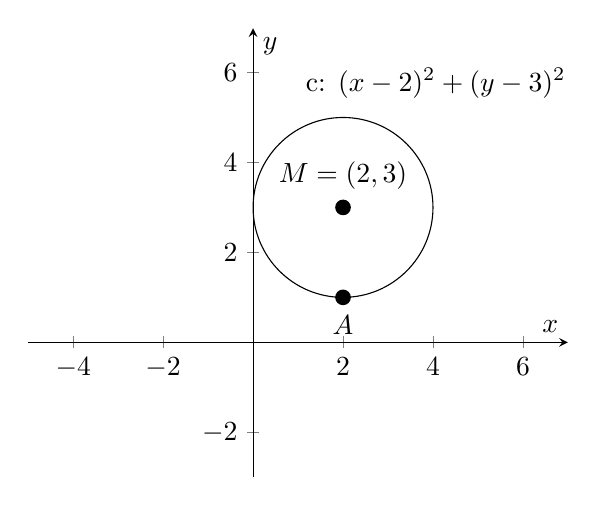
\begin{tikzpicture}
\begin{axis}[xmin=-5, xmax=7, ymin=-1, ymax=5,
axis lines = middle,xlabel=$x$,ylabel=$y$, axis equal]
\draw (axis cs: 2, 3) circle [radius=2];
%	\addplot[red,mark=*] coordinates {(2,3)};
\node[label={90:{$M=(2,3)$}},circle,fill,inner sep=2pt] at (axis cs:2,3) {};
\node[label={270:{$A$}},circle,fill,inner sep=2pt] at (axis cs:2,1) {};
\node[label={90:{c: $(x-2)^2+(y-3)^2=4$}},xshift=1.5cm] at (axis cs:2,5) {};
\end{axis}

%	\begin{axis}[
%	axis lines = left,
%	xmin=-11, xmax=11, ymin=-11, ymax=11,
%	axis equal,
%	xlabel = $x$,
%	ylabel = {$f(x)$},
%	yticklabels={,,}
%	]
%	\draw (axis cs: 0, 0) circle [radius=10];% I've set the radius to 10 only for better show the image
%	\end{axis}

\end{tikzpicture}
\end{center}

%\gewonefiguur{height=7cm}{4_opp_inhoud_an_meetk/inputs/AMTekst7Fig1}

%\begin{figure}[h]
%\begin{center}
%\includegraphics[height=5 cm]{4_opp_inhoud_an_meetk/inputs/AMTekst7Fig1}
%\caption{}
%\label{fig4.2.15_fig1}
%\end{center}
%\end{figure}

Bovenstaande figuur stelt de cirkel voor met middelpunt $M(2;3)$ en straal $r=2$.
Dit is dus de cirkel $C((2;3),2)$.\\

Uit de formule voor de afstand tussen twee punten in het vlak (met Euclidische co\"ordinaten) vinden we dat een punt $P(x;y)$ behoort tot de cirkel $C(M,r)$ met $M(x_0;y_0)$ als en alleen als
\[
\sqrt {(x-x_0)^2+(y-y_0)^2}=r \text { .}
\]
Omdat beide leden van deze vergelijking positief zijn is deze voorwaarde geldig als en alleen als de gelijkheid tussen de kwadraten van beide leden geldt.
We bekomen dan volgende vergelijking voor de cirkel $C(M,r)$:
\[
(x-x_0)^2+(y-y_0)^2=r^2 \text { .}
\]
Deze vergelijking zie je ook ingevuld in de tekening.

\begin{voorbeeld}
	De vergelijking van de cirkel met middelpunt $M(1;4)$ en straal 5 is
\[
(x-1)^2+(y-4)^2=25 \text { .}
\]
\end{voorbeeld}
\begin{voorbeeld}
	De vergelijking van de cirkel met middelpunt $O(0;0)$ en straal 4 is
\[
x^2+y^2=16 \text { .}
\]
\end{voorbeeld}
\begin{voorbeeld}
	De goniometrische cirkel is de cirkel met middelpunt $O(0;0)$ en straal 1.
De vergelijking van de goniometrische cirkel is
\[
x^2+y^2=1 \text { .}
\]

\end{voorbeeld}

\vspace{2mm} Stel dat $C$ een cirkel is met middelpunt $M$ en $P$ een punt $C$.
De raaklijn $T$ aan $C$ in $P$ staat loodrecht op de straal $MP$.
Dit kun je gebruiken om de vergelijking op de stellen van een raaklijn aan een cirkel.

%\underline{Voorbeeld:} Gegeven is de cirkel $C$ met middelpunt $M(1;2)$ en straal 3.
%Stel vergelijkingen op voor de raaklijnen aan $C$ in de snijpunten van $C$ met de $x$-as.
%
%De vergelijking van $C$ is $(x-1)^2+(y-2)^2=9$.
%Omdat $y=0$ voor een punt op de $x$-as voldoet de $x$-co\"ordinaat van het snijpunt van $C$ met de $x$-as aan de vergelijking
%\[
%(x-1)^2+4=9 \text { dus } (x-1)^2=5 \text { dus } x-1=\pm \sqrt {5}
%\]
%en je bekomt twee oplossingen $x=1 \pm \sqrt {5}$.
%De snijpunten van $C$ met de $x$-as hebben co\"ordinaten $P_1(1-\sqrt {5};0)$ en $P_2(1+\sqrt {5};0)$.
%
%Er geldt $\rico (MP_1)=\frac {2}{1-(1-\sqrt {5})}=\frac {2}{\sqrt {5}}$.
%De richtingsco\"effici\"ent van de raaklijn $T_1$ aan $C$ in $P_1$ is gelijk aan $-\frac {\sqrt {5}}{2}$.
%De vergelijking van $T_1$ is
%\[
%y=-\frac {\sqrt {5}}{2}(x-(1-\sqrt {5}))=-\frac {\sqrt {5}}{2}x+\left( \frac {\sqrt { 5}}{2}-\frac {5}{2}  \right) \text { .}
%\]
%
%Er geldt $\rico (MP_2)=\frac {2}{1-(1+\frac {5})}=-\frac {2}{\sqrt {5}}$.
%De richtingsco\"effici\"ent van de raaklijn $T_2$ aan $C$ in $P_2$ is gelijk aan $\frac {\sqrt {5}}{2}$.
%De vergelijking van $T_2$ is
%\[
%y=\frac {\sqrt {5}}{2}(x-(1+\sqrt {5}))=\frac {\sqrt {5}}{2}x-\left( \frac {\sqrt { 5}}{2}+\frac {5}{2}  \right) \text { .}
%\]\\
%
%Een omgeschreven cirkel van een driehoek is een cirkel die door alle hoekpunten van de driehoek gaat.
%\begin{figure}[h]
%\begin{center}
%\includegraphics[height=5 cm]{4_opp_inhoud_an_meetk/inputs/AMTekst7Fig3}
%\caption{}
%\label{fig4.2.15_fig3}
%\end{center}
%\end{figure}
%Het is de cirkel met minimale oppervlakte waarbinnen de driehoek ligt.
%
%Het middelpunt $M$ ligt evenver van de drie hoekpunten $K$, $H$ en $I$ van de driehoek.
%Omdat $M$ evenver van $K$ als $H$ ligt behoort $M$ tot de middelloodlijn op het lijnstuk $[K;H]$.
%In het bijzonder gaan de drie middelloodlijnen van de driehoek door eenzelfde punt (het middelpunt $M$ van de omgeschreven cirkel).
%De afstand van dat punt $M$ tot \'e\'en van de hoekpunten is de straal van de omgeschreven cirkel.\\

\begin{voorbeeld}
	$\Delta$ is de driehoek met hoekpunten $A(-3;-1)$, $B(1;4)$ en $C(2;-3)$.
Stel een vergelijking op van de omgeschreven cirkel van $\Delta$.

\begin{center}
	\tikzsetfigurename{module4_2_14_vglCirkelVb}
	\begin{tikzpicture}
\draw[->] (-5,0)--(5,0) node[anchor=south,left,yshift=0.2cm]{$x$};
\draw[->] (0,-4)--(0,6) node[anchor=south,left]{$y$};

\tkzDefPoint(0,0){S}
\tkzDefPoint(1,0){x1}
\tkzDefPoint(0,1){y1}

\tkzDefPoint(-3,0){A1}
\tkzDefPoint(0,-1){A2}

\tkzDefPoint(-3,-1){A}

\tkzDefPoint(1,0){B1}
\tkzDefPoint(0,4){B2}

\tkzDefPoint(1,4){B}

\tkzDefPoint(2,0){C1}
\tkzDefPoint(0,-3){C2}

\tkzDefPoint(2,-3){C}

\tkzLabelPoint[below,xshift=-0.1cm](S){$0$}
%	\tkzLabelPoint[right,yshift=-0.3cm](S){$O$}

\tkzLabelPoint[below](x1){$1$}
\tkzLabelPoint[left](y1){$1$}

\tkzLabelPoint[left,yshift=0.2cm](A){$A$}
\tkzLabelPoint[right,yshift=0.2cm](B){$B$}
\tkzLabelPoint[right,yshift=0.2cm](C){$C$}

\tkzLabelPoint[above](A1){$-3$}
\tkzLabelPoint[right](A2){$-1$}

%	\tkzLabelPoint[below](B1){$-1$}
\tkzLabelPoint[left](B2){$4$}

\tkzLabelPoint[above](C1){$2$}
\tkzLabelPoint[left](C2){$-3$}	

\tkzDrawSegment[black!60!black,dotted](A1,A)
\tkzDrawSegment[black!60!black,dotted](A2,A)
\tkzDrawSegment[black!60!black,dotted](B1,B)
\tkzDrawSegment[black!60!black,dotted](B2,B)
\tkzDrawSegment[black!60!black,dotted](C1,C)
\tkzDrawSegment[black!60!black,dotted](C2,C)

\tkzDrawSegment[black!60!black](A,C)
\tkzDrawSegment[black!60!black](A,B)
\tkzDrawSegment[black!60!black](B,C)

\foreach \n in {S,x1,y1,A1,A2,A,B1,B2,B,C1,C2,C}
\node at (\n)[circle,fill,inner sep=1.5pt]{};

\end{tikzpicture}
\end{center}


%\gewonefiguur{height=7cm}{4_opp_inhoud_an_meetk/inputs/AMTekst7Fig2}

%\begin{figure}[h]
%\begin{center}
%\includegraphics[width=.5\linewidth]{4_opp_inhoud_an_meetk/inputs/AMTekst7Fig2}
%\caption{}
%\label{fig4.2.15_fig2}
%\end{center}
%\end{figure}

Omdat het middelpunt $M$ het snijpunt is van de middelloodlijnen van $\Delta$ berekenen we eerst twee middelloodlijnen van $\Delta$.
De middelloodlijn van het lijnstuk $[A;B]$ is de verzameling van de punten $P(x;y)$ die evenver van $A$ als van $B$ liggen.
Als we $d(P;A)^2=d(P;B)^2$ in co\"ordinaten uitdrukken bekomen we
\[
(x+3)^2+(y+1)^2=(x-1)^2+(y-4)^2 \text { .}
\]
Door de machten uit te werken en te vereenvoudigen bekom je
\[
8x+10y-7=0 \text { .}
\]
Dit is de vergelijking van de middelloodlijn $m_C$ van de zijde $BC$ van $\Delta$.

Door $d(P;A)^2=d(P;C)^2$ in co\"ordinaten uit te schrijven bekom je
\[
(x+3)^2+(y+1)^2=(x-2)^2+(y+3)^2 \text { .}
\]
Hieruit bekom je
\[
10x-4y+3=0 \text { .}
\]
Dit is de vergelijking van de middelloodlijn $m_B$ van de zijde $AC$ van $\Delta$.

De co\"ordinaten van het middelpunt $M(x_0;y_0)$ van de omgeschreven cirkel van $\Delta$ is de oplossing van het stelsel
\[
\begin{cases}
8x+10y-7=0\\
10x-4y+3=0
\end{cases}
\]
Lossen we beide vergelijkingen op naar $y$ dan bekomen we
\[
\begin{cases}
y=-\frac {8}{10}x+\frac {7}{10}\\
y=\frac {10}{4}x-\frac {3}{4}
\end{cases}
\]
Hieruit volgt dat $x_0$ de oplossing is van de vergelijking
\[
-\frac {8}{10}x+\frac {7}{10}=\frac {10}{4}x-\frac {3}{4} \text { .}
\]
Hieruit bekom je dat $x_0=\frac {29}{66}=0,44$.
Vul je dit in $y=-\frac {8}{10}x+\frac {7}{10}$ is dan bekom je $y_0$, dus
\[
y_0=-\frac {8}{10}.\frac {29}{66}+\frac {7}{10}=\frac {23}{66}=0,35 \text { .}
\]
Het middelpunt $M$ van de omgeschreven cirkel van $\Delta$ is $M(0,44;0,35)$.

De straal $r$ van de omgeschreven cirkel is de afstand van $M$ tot $A$:
\[
r=d(M;A)=\sqrt {\left(  -3-\frac {29}{66} \right)^2+\left( -1-\frac {23}{66} \right)^2}=3,69 \text { .}
\]
Je rekent zelf na dat dit ook $d(M;B)$ en $d(M;C)$ is.

De vergelijking van de omgeschreven cirkel is dus
\[
(x-0,44)^2+(y-0,35)^2=3,69^2=13,62 \text { .}
\]\\

Een ingeschreven cirkel van een driehoek is een cirkel binnen de driehoek die raakt aan de drie zijden van de driehoek.

\begin{center}
	\tikzsetfigurename{module4_2_14_ingeschrevenCirkel}
	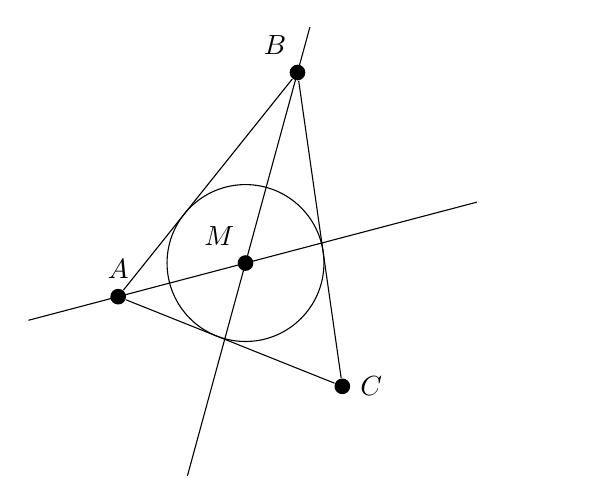
\begin{tikzpicture}
\begin{axis}[xmin=-5, xmax=7, ymin=-5, ymax=5,
axis lines = middle,xlabel=\empty,ylabel=\empty, axis equal, axis line style={draw=none},
xtick=\empty, ytick=\empty,
tick style={draw=none},
domain=-5:5,
samples=101,
smooth,
no markers]
\draw (axis cs: -0.16, -0.25) circle [radius=1.75];
%	\addplot[red,mark=*] coordinates {(2,3)};
\node[label={100:{$M$}},circle,fill,inner sep=2pt] at (axis cs:-0.16,-0.25) {};
\node[label={90:{$A$}},circle,fill,inner sep=2pt] (A) at (axis cs:-3,-1) {};
\node[label={100:{$B$}},circle,fill,inner sep=2pt] (B) at (axis cs:1,4) {};
\node[label={0:{$C$}},circle,fill,inner sep=2pt] (C) at (axis cs:2,-3) {};
%	\node[label={270:{$A$}},circle,fill,inner sep=2pt] at (axis cs:2,1) {};

\draw[-](A)--(B);
\draw[-](B)--(C);
\draw[-](C)--(A);

\addplot[black] {14.11/53.556*x-11.198/53.556};
\addplot[black] {80.177/21.881*x+7.347/21.881};

\end{axis}

%	\draw[->] (-5,0)--(5,0) node[anchor=south,left,yshift=0.2cm]{$x$};
%	\draw[->] (0,-4)--(0,6) node[anchor=south,left]{$y$};
%	
%	\tkzDefPoint(0,0){S}
%	\tkzDefPoint(1,0){x1}
%	\tkzDefPoint(0,1){y1}
%	
%	\tkzDefPoint(-3,0){A1}
%	\tkzDefPoint(0,-1){A2}
%	
%	\tkzDefPoint(-3,-1){A}
%	
%	\tkzDefPoint(1,0){B1}
%	\tkzDefPoint(0,4){B2}
%	
%	\tkzDefPoint(1,4){B}
%	
%	\tkzDefPoint(2,0){C1}
%	\tkzDefPoint(0,-3){C2}
%	
%	\tkzDefPoint(2,-3){C}
%	
%	\tkzLabelPoint[below,xshift=-0.1cm](S){$0$}
%	%	\tkzLabelPoint[right,yshift=-0.3cm](S){$O$}
%	
%	\tkzLabelPoint[below](x1){$1$}
%	\tkzLabelPoint[left](y1){$1$}
%	
%	\tkzLabelPoint[left,yshift=0.2cm](A){$A$}
%	\tkzLabelPoint[right,yshift=0.2cm](B){$B$}
%	\tkzLabelPoint[right,yshift=0.2cm](C){$C$}
%	
%	\tkzLabelPoint[above](A1){$-3$}
%	\tkzLabelPoint[right](A2){$-1$}
%	
%	%	\tkzLabelPoint[below](B1){$-1$}
%	\tkzLabelPoint[left](B2){$4$}
%	
%	\tkzLabelPoint[above](C1){$2$}
%	\tkzLabelPoint[left](C2){$-3$}	
%	
%	\tkzDrawSegment[black!60!black,dotted](A1,A)
%	\tkzDrawSegment[black!60!black,dotted](A2,A)
%	\tkzDrawSegment[black!60!black,dotted](B1,B)
%	\tkzDrawSegment[black!60!black,dotted](B2,B)
%	\tkzDrawSegment[black!60!black,dotted](C1,C)
%	\tkzDrawSegment[black!60!black,dotted](C2,C)
%	
%	\tkzDrawSegment[black!60!black](A,C)
%	\tkzDrawSegment[black!60!black](A,B)
%	\tkzDrawSegment[black!60!black](B,C)
%	
%	\foreach \n in {S,x1,y1,A1,A2,A,B1,B2,B,C1,C2,C}
%	\node at (\n)[circle,fill,inner sep=1.5pt]{};

\end{tikzpicture}
\end{center}

%\gewonefiguur{height=5cm}{4_opp_inhoud_an_meetk/inputs/AMTekst7Fig3}

%\begin{figure}[h]
%\begin{center}
%\includegraphics[height=5 cm]{4_opp_inhoud_an_meetk/inputs/AMTekst7Fig3}
%\caption{}
%\label{fig4.2.15_fig3}
%\end{center}
%\end{figure}
Het is de cirkel met maximale oppervlakte die binnen de driehoek ligt.

Noem $M$ het middelpunt van die cirkel.
Omdat iedere zijde van de driehoek een raaklijn aan de cirkel is en omdat de bijbehorende straal van cirkel (lijnstuk van M naar de zijde) loodrecht staat op de zijde is de afstand van $M$ tot een zijde van de driehoek de straal $r$ van de cirkel.
Omdat deze afstand voor iedere zijde gelijk is ligt $M$ evenver van iedere zijde van de driehoek.
Hieruit bekom je dat $M$ evenver ligt van iedere twee zijden van de driehoek en dus voor iedere twee zijden van de driehoek op een bissectrice ligt.
Omdat $M$ eveneens binnen de driehoek moet liggen moet $M$ voor iedere twee zijden van driehoek gelegen zijn op de binnenbissectrice (diegene die de hoek van driehoek in twee gelijke delen verdeelt).
Je vindt daarom $M$ door twee binnenbissectrices van de driehoek te berekenen de daarvan het snijpunt te bepalen.
De straal is dan de afstand van $M$ tot eender welke zijde van de driehoek.\\

\end{voorbeeld}

\begin{voorbeeld}
	Voor de driehoek $\Delta$ uit het vorige voorbeeld stel je een vergelijking op van de ingesloten cirkel.

Omdat we binnenbissectrices van $\Delta$ (dus bissectrices van de zijden van $\Delta$) gaan we eerst vergelijkingen van de zijden van de driehoek opstellen.
Door de formule voor een vergelijking van een rechte door twee gegeven punten te gebruiken bekom je de volgende vergelijkingen:
\[
AB \leftrightarrow 5x-4y+11=0
\]
\[
AC \leftrightarrow 2x+5y+11=0
\]
\[
BC \leftrightarrow 7x+y-11=0
\]

Een bissectrice tussen $AB$ en $AC$ is gegeven door volgende vergelijking
\[
\frac {5x-4y+11}{\sqrt {25+16}}=\frac {2x+5y+11}{\sqrt {4+25}}
\]
\[
(5\sqrt {29}-2\sqrt{41})x+(-4\sqrt{29}-5\sqrt{41})y+(11\sqrt{29}-11\sqrt{41})=0 \text { .}
\]
Je rekent na dat de richtingsco\"effici\"ent van deze bissectrice gelijk is aan 0,26.
Deze bissectrice is dus een licht stijgende rechte.
Dit komt overeen met de tekening, dit is dus een vergelijking van een binnenbissectrice $b_A$ van de driehoek.

Een bissectrice van $AB$ en $BC$ is gegeven door volgende vergelijking
\[
\frac {5x-4y+11}{\sqrt {25+16}}=\frac {7x+y-11}{\sqrt {49+1}}
\]
\[
(5\sqrt {50}-7\sqrt {41})x+(-4\sqrt {50}-\sqrt {41})y+(11 \sqrt{50}+11\sqrt {41})=0 \text { .}
\]
Je rekent na dat de richtingsco\"effici\"ent van deze bissectrice gelijk is aan $-0,27$.
Deze bissectrice is een licht dalende rechte.
Dit komt niet overeen met de tekening, het is dus niet een binnenbissectrice van de driehoek.

De binnenbissectrice heeft daarom vergelijking
\[
\frac {5x-4y+11}{\sqrt {25+16}}=-\frac {7x+y-11}{\sqrt {49+1}}
\]
\[
(5\sqrt {50}+7\sqrt {41})x+(-4\sqrt {50}+\sqrt {41})y+(11 \sqrt{50}-11\sqrt {41})=0 \text { .}
\]

De co\"ordinaten van het middelpunt $M(x_0;y_0)$ van de ingeschreven cirkel is de oplossing van het stelsel vergelijkingen
\[
\begin{cases}
(5\sqrt {29}-2\sqrt{41})x+(-4\sqrt{29}-5\sqrt{41})y+(11\sqrt{29}-11\sqrt{41})=0 \\
(5\sqrt {50}+7\sqrt {41})x+(-4\sqrt {50}+\sqrt {41})y+(11 \sqrt{50}-11\sqrt {41})=0
\end{cases}
\]
Na enig rekenwerk bekom je $M(-0,16;-0,25)$.

De straal $r$ van de ingeschreven cirkel is de afstand van $M$ tot de rechte $AB$.
Je bekomt
\[
r=\frac {\vert 5.(-0,16)-4.(-0,25)+11 \vert }{\sqrt {25+16}}=1,75 \text { .}
\]
Je rekent zelf na dat die ook de afstand van $M$ tot de rechte $AC$ en van $M$ tot de rechte $BC$ is.

De vergelijking van de ingeschreven cirkel is
\[
(x+0,16)^2+(y+0,25)^2=1,75^2=3,06 \text { .}
\]

\end{voorbeeld}